% Hamiltonian Predictive Coding
%
% Formatted with the standard `article` class so it compiles anywhere.
% FOR NeurIPS SUBMISSION: delete the geometry/font block marked below and
% replace it with   \usepackage[final]{neurips_2025}   (download the style
% file from the NeurIPS site). The body needs no other changes.
\documentclass[10pt]{article}

% ---- begin replaceable layout block (swap for neurips_2025.sty) ----------
% For NeurIPS submission, replace this whole block with:
%     \usepackage[final]{neurips_2025}
% (neurips_2025.sty loads natbib itself, so it is included here for the
%  standalone build and removed along with this block.)
\usepackage[margin=1in]{geometry}
\usepackage{times}
\usepackage{natbib}
\renewcommand{\baselinestretch}{1.02}
% ---- end replaceable layout block ----------------------------------------

\usepackage{amsmath,amssymb,amsthm}
\usepackage{graphicx}
\usepackage{booktabs}
\usepackage{xcolor}
\usepackage{microtype}
\usepackage[colorlinks=true,allcolors=blue]{hyperref}

\graphicspath{{../figures/}}

\newtheorem{theorem}{Theorem}
\newtheorem{proposition}{Proposition}
\theoremstyle{remark}
\newtheorem{remark}{Remark}

\newcommand{\R}{\mathbb{R}}
\newcommand{\bz}{\mathbf{z}}
\newcommand{\bpi}{\boldsymbol{\pi}}
\newcommand{\bPhi}{\boldsymbol{\Phi}}
\newcommand{\bW}{\mathbf{W}}
\newcommand{\bu}{\mathbf{u}}
\newcommand{\eps}{\epsilon}
\newcommand{\grad}{\nabla}
\newcommand{\half}{\tfrac{1}{2}}

\title{\bf Hamiltonian Predictive Coding:\\
Local, Energy-Based Credit Assignment through Time-Reversal Symmetry}

\author{Anonymous Author(s)\\ Affiliation\\ \texttt{email}}
\date{}

\begin{document}
\maketitle

\begin{abstract}
Predictive coding (PC) is a leading candidate for a biologically plausible
and hardware-friendly alternative to backpropagation: it learns with a local
Hebbian rule driven by prediction errors. Yet two frictions persist. Its
inference is a dissipative relaxation to equilibrium that must converge
before every weight update, and its temporal credit assignment for sequence
data is either heuristic or falls back to backpropagation through time
(BPTT), forfeiting locality. We show that both frictions dissolve when the PC
free energy is treated as the potential energy of a \emph{conservative}
dynamical system. Endowing the value units with momenta turns the entire PC
hierarchy into a single Hamiltonian recurrent unit whose inference is one
symplectic forward pass and whose learning is \emph{Recurrent Hamiltonian
Echo Learning} (RHEL): two additional momentum-flipped ``echo'' passes whose
trajectory contrast encodes the loss gradient. We prove that for the PC
Hamiltonian this contrast \emph{is exactly} the predictive-coding Hebbian
rule---an error\,$\times$\,activity outer product---computed forward in time,
using the same weights in the forward and backward passes (no weight
transport), and equal to BPTT in the small-nudge limit. Empirically, on a
hierarchical Hamiltonian PC network we find: (i) RHEL gradients match BPTT to
machine precision and decompose into the local rule at every layer
($\cos=1.0$, residual $\sim\!10^{-8}$); (ii) the network learns a generative
model with no labels, reducing held-out reconstruction error $12\times$ below
a random reservoir while the local rule tracks global BPTT step for step; and
(iii) the symmetric two-echo estimator has $O(\eps^2)$ bias versus $O(\eps)$
for the one-sided Equilibrium-Propagation estimator. Hamiltonian predictive
coding thus realizes inference and learning as one conservative physical
process with a fully local plasticity rule, pointing toward self-learning
predictive-coding machines.
\end{abstract}

\section{Introduction}
\label{sec:intro}

The resurgence of recurrent and state-space sequence models has reopened the
question of whether learning must be tied to the GPU/backpropagation
paradigm, or whether neural computation could instead be embodied in physical
dynamical systems endowed with their own credit-assignment mechanisms
\citep{rhel,physnn,hardwarelottery}. Two desiderata recur for such
``self-learning machines'': learning should use \emph{forward passes only}
(no separate backward solver), and it should avoid the explicit state
Jacobian \citep{rhel}.

Predictive coding (PC) is one of the most studied biologically motivated
learning frameworks \citep{raoballard,whittingtonbogacz}. A PC network is a
generative hierarchy in which each level predicts the level below; only
prediction errors propagate, and weights are updated by a \emph{local} Hebbian
rule---the product of a prediction error and a presynaptic activity. This
locality is precisely what makes PC attractive for neuromorphic and analog
substrates. Yet classical PC has frictions that the physical-learning agenda
exposes. First, its inference is a \emph{dissipative} relaxation: value units
descend the free energy to an equilibrium that must (approximately) converge
before each weight update. Second, applying PC to \emph{sequences} requires
either an ad-hoc temporal recurrence or a fallback to backpropagation through
time (BPTT), which sacrifices the very locality that motivated PC. Third, the
classic equivalence of PC to backpropagation is asymptotic and contingent on
inference convergence \citep{whittingtonbogacz,millidge_review}.

Independently, \citet{rhel} introduced Recurrent Hamiltonian Echo Learning
(RHEL), a forward-only proxy of BPTT for \emph{non-dissipative Hamiltonian}
systems. RHEL exploits time-reversal symmetry: flipping the momenta at the
end of a trajectory makes a conservative system retrace its history, and a
small loss-dependent nudge of this reverse ``echo'' makes the trajectory
deviate by exactly the adjoint state. Gradients fall out as finite
differences of two echo trajectories---three forward passes, no Jacobian,
provably equal to BPTT.

\paragraph{Contributions.} We bring these two threads together. Our claim is
that predictive coding is the \emph{natural} model class for RHEL, and that
the combination---\emph{Hamiltonian Predictive Coding} (HPC)---resolves PC's
frictions while sharpening RHEL into a manifestly local rule.
\begin{itemize}
\item \textbf{Construction (\S\ref{sec:hpc}).} Treating the PC free energy as
potential energy and giving value units momenta turns the whole hierarchy
into a single Hamiltonian recurrent unit. Inference becomes one symplectic
(leapfrog) forward pass; no relaxation to equilibrium is required.
\item \textbf{Locality (\S\ref{sec:hpc}, \S\ref{sec:locality}).} We prove
(Prop.~\ref{prop:local}) that the RHEL update for the PC Hamiltonian is
exactly the PC Hebbian rule---a contrast of error\,$\times$\,activity outer
products over the two echoes---using the \emph{same} weights forward and
backward (no weight transport) and equal to BPTT as $\eps\!\to\!0$. We confirm
this numerically to $\sim\!10^{-8}$ and contrast it with backpropagation's
dependence on transported weights.
\item \textbf{Energy-based unsupervised learning (\S\ref{sec:unsup}).} Because
PC is generative, HPC learns with no labels by minimizing its free energy. It
reduces held-out reconstruction error $12\times$ below a random reservoir,
and the local RHEL rule matches global BPTT step for step.
\item \textbf{The nudging knob (\S\ref{sec:knob}).} RHEL is a one-parameter
family interpolating between an exact BPTT proxy ($\eps\!\to\!0$) and a robust
contrastive estimator. We show the symmetric two-echo (centered) estimator
has $O(\eps^2)$ bias versus $O(\eps)$ for the one-sided
Equilibrium-Propagation estimator, and identify the finite-precision sweet
spot.
\end{itemize}
We are explicit about the cost of conservativity: non-dissipative inference
cannot forget, which constrains both tasks and the choice of leak
(\S\ref{sec:limitations}).

\section{Background}
\label{sec:background}

\paragraph{Predictive coding.} Consider a hierarchy of value vectors
$\bz=(\bz_0,\dots,\bz_{L-1})$, a clamped input $\bu$, an elementwise
nonlinearity $f$, and generative weights $\theta=\{\bW_0,\dots,\bW_{L-1}\}$.
With prediction errors
\begin{equation}
\label{eq:errors}
\mathbf{e}_0 = \bu - \bW_0 f(\bz_0), \qquad
\mathbf{e}_\ell = \bz_{\ell-1} - \bW_\ell f(\bz_\ell)\ \ (\ell=1,\dots,L-1),
\end{equation}
the free energy is
$F(\bz;\theta,\bu)=\sum_{\ell=0}^{L-1}\half\|\mathbf{e}_\ell\|^2
+\tfrac{\alpha}{2}\|\bz\|^2$,
with $\alpha$ a leak. Classical PC performs inference by gradient
relaxation $\dot{\bz}=-\grad_{\bz}F$ to an equilibrium $\bz^\star$, then
applies the local Hebbian update
\begin{equation}
\label{eq:pc_hebb}
\Delta \bW_\ell \;\propto\; \mathbf{e}_\ell\, f(\bz_{\ell+1})^{\!\top}
\quad\text{at } \bz^\star,
\end{equation}
which needs only the error at the synapse's output and the activity at its
input \citep{raoballard,whittingtonbogacz}.

\paragraph{Hamiltonian recurrent units and RHEL.}
\citet{rhel} consider a system with position $\boldsymbol{\phi}$ and momentum
$\bpi$, state $\bPhi=(\boldsymbol{\phi},\bpi)$, and a separable, time-reversal
invariant Hamiltonian $H[\bPhi,\theta,\bu]=T[\bpi]+V[\boldsymbol{\phi}]$
integrated by the symplectic leapfrog map $M_{H,\delta}=M_{T,\delta/2}\circ
M_{V,\delta}\circ M_{T,\delta/2}$, which is \emph{exactly} time-reversible. A
Hamiltonian recurrent unit (HRU) is such an integrator run over an input
sequence. Given a loss $L=\sum_k \ell[\bPhi_k,k]$, RHEL runs, after the free
forward pass, two ``echo'' passes that start from the momentum-flipped final
state, replay the inputs in reverse, and are nudged by $\pm\eps\,\grad\ell$.
The parameter gradient is read out as a finite difference of the Hamiltonian
gradients along the two echoes,
\begin{equation}
\label{eq:rhel}
\Delta_\theta(k,\eps) = -\frac{\delta}{2\eps}\Big(
\grad_\theta H^{1/2}[\bPhi^e_k(\eps)] - \grad_\theta H^{1/2}[\bPhi^e_k(-\eps)]\Big),
\end{equation}
where $H^{1/2}$ is the Hamiltonian at the intermediate leapfrog states. The
central guarantee is exactness.
\begin{theorem}[\citealp{rhel}, Thm.~3.2, informal]
\label{thm:rhel}
For an HRU with a separable, time-reversal-invariant Hamiltonian and a
twice-differentiable loss, RHEL equals BPTT at every step:
$\lim_{\eps\to0}\Delta_\theta(k,\eps)=\mathrm{d}_\theta L$, with no state
Jacobian and using only forward simulations of the dynamics.
\end{theorem}

\section{Hamiltonian Predictive Coding}
\label{sec:hpc}

\begin{figure}[t]
\centering
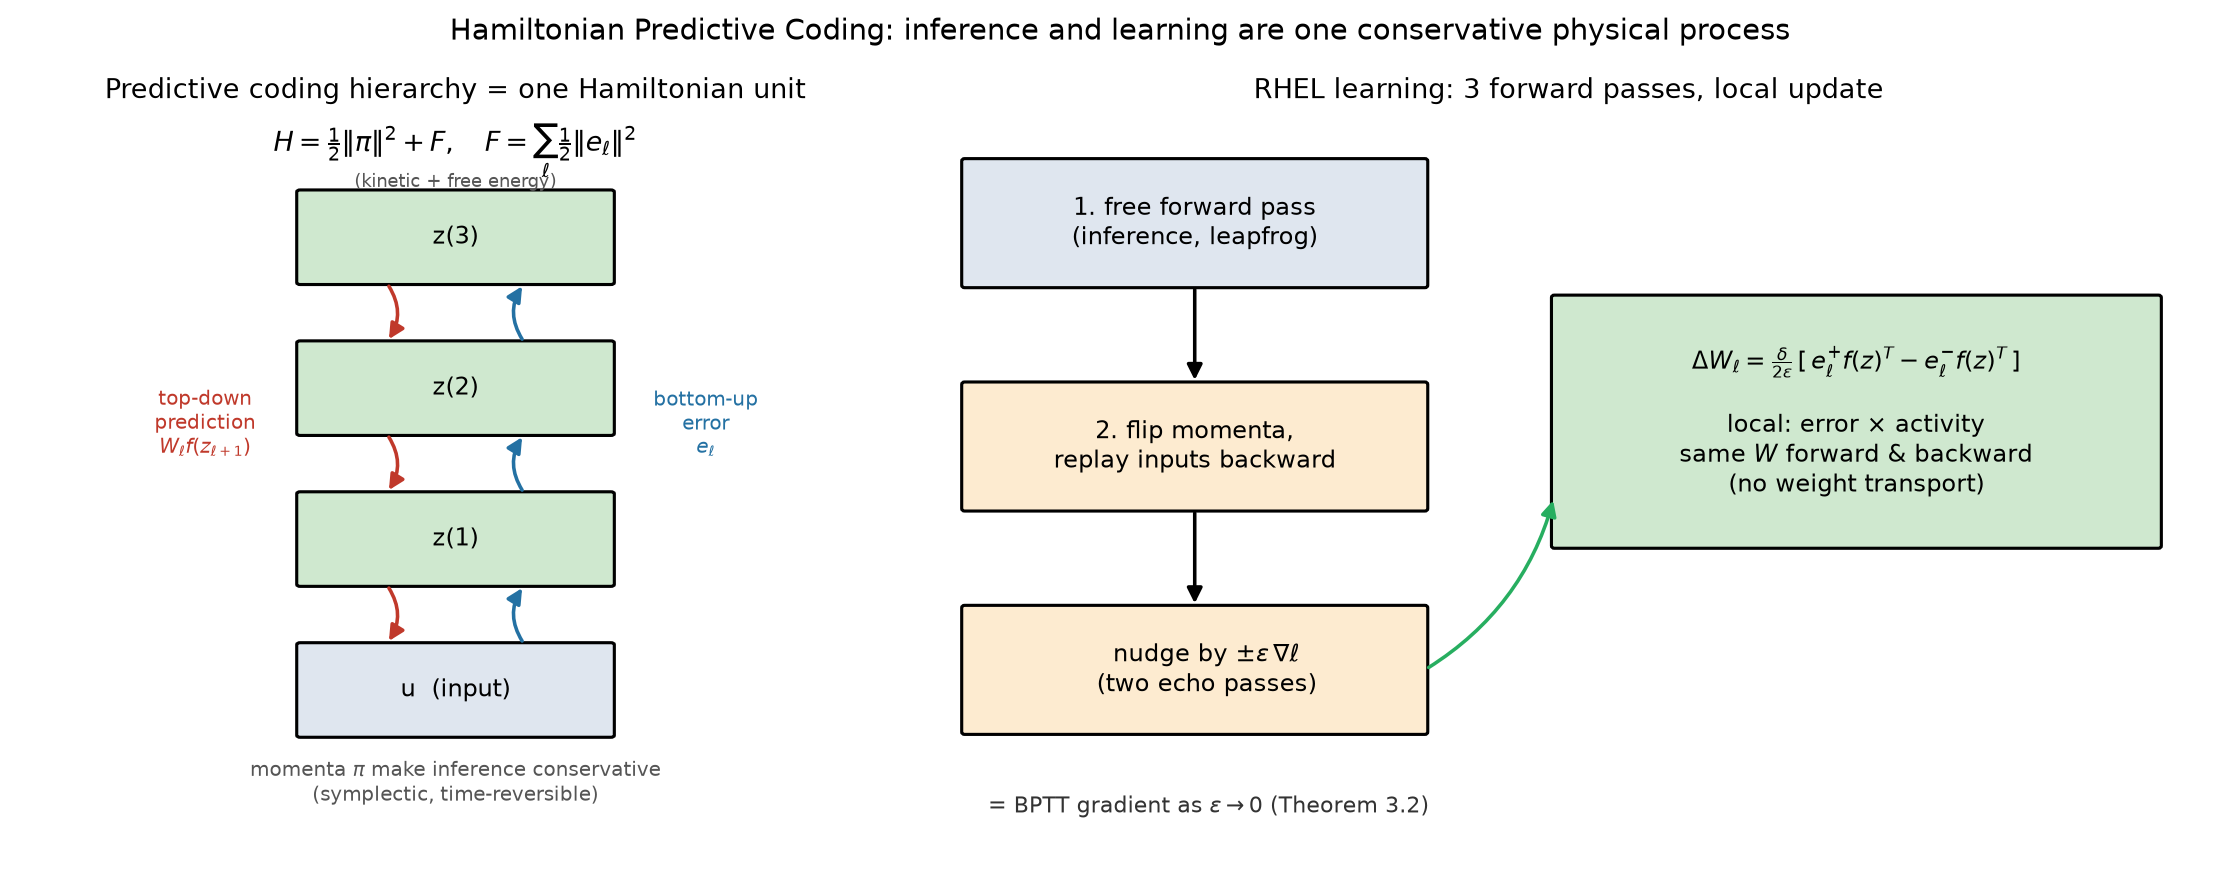
\includegraphics[width=\linewidth]{concept_schematic.png}
\caption{\textbf{Hamiltonian predictive coding.} \emph{Left:} the PC
hierarchy with top-down predictions $\bW_\ell f(\bz_{\ell+1})$ and bottom-up
errors $\mathbf{e}_\ell$; giving the value units momenta makes the free
energy $F$ the potential of a conservative, time-reversible system.
\emph{Right:} learning is RHEL---one free forward (inference) pass and two
momentum-flipped echo passes nudged by $\pm\eps$; the per-synapse update is
the local error\,$\times$\,activity contrast across the echoes, uses the same
weights forward and backward, and equals the BPTT gradient as
$\eps\!\to\!0$.}
\label{fig:concept}
\end{figure}

\paragraph{The model.} Endow each value unit with a conjugate momentum $\bpi$
and define the separable Hamiltonian
\begin{equation}
\label{eq:hpc_H}
H[\bPhi,\theta,\bu] \;=\; \underbrace{\half\|\bpi\|^2}_{T[\bpi]}
\;+\; \underbrace{F(\bz;\theta,\bu)}_{V[\bz]},
\qquad \bPhi=(\bz,\bpi).
\end{equation}
Hamilton's equations give second-order inference dynamics
$\dot{\bz}=\bpi,\ \dot{\bpi}=-\grad_{\bz}F$, i.e. $\ddot{\bz}=-\grad_{\bz}F$:
the prediction-error forces of PC now act as restoring forces on oscillating
units rather than as a relaxation. Because $T$ depends only on $\bpi$ and $V$
only on $\bz$, and both are even under momentum flip, $H$ is separable and
time-reversal invariant, so the leapfrog integrator is reversible and
Theorem~\ref{thm:rhel} applies. The whole hierarchy is thus a single HRU
driven at its sensory layer by $\bu_k$; inference is one forward pass, with
\emph{no} inner relaxation loop.

\paragraph{Learning is the PC Hebbian rule.} For the PC potential, the
Hamiltonian gradient with respect to a generative weight is itself local:
$\grad_{\bW_\ell}H=\grad_{\bW_\ell}F=-\mathbf{e}_\ell f(\bz_\ell)^{\!\top}$.
Substituting into~\eqref{eq:rhel} yields our central observation.
\begin{proposition}[RHEL realizes the PC Hebbian rule]
\label{prop:local}
For the Hamiltonian~\eqref{eq:hpc_H}, the RHEL update for $\bW_\ell$ is
\begin{equation}
\label{eq:hpc_update}
\Delta \bW_\ell \;=\; \frac{\delta}{2\eps}\sum_k\Big(
\mathbf{e}_\ell^{+}(k)\, f(\bz_\ell^{+}(k))^{\!\top}
- \mathbf{e}_\ell^{-}(k)\, f(\bz_\ell^{-}(k))^{\!\top}\Big),
\end{equation}
where $\pm$ denote quantities along the $\pm\eps$ echo trajectories. Each term
is a (prediction error at the synapse output)\,$\times$\,(activity at the
synapse input) outer product---the classic PC plasticity signal
\eqref{eq:pc_hebb}---and uses the same weights $\bW_\ell$ as the forward pass.
By Theorem~\ref{thm:rhel}, $\lim_{\eps\to0}\Delta\bW_\ell=\mathrm{d}_{\bW_\ell}L$.
\end{proposition}
Equation~\eqref{eq:hpc_update} is the crux: RHEL turns PC's
equilibrium Hebbian rule into a \emph{contrastive} Hebbian rule evaluated
along two physical echo trajectories, with no equilibrium, no weight
transport, and no separate error network---inference and learning are one
conservative process (Fig.~\ref{fig:concept}). Table~\ref{tab:compare}
summarizes the differences from classical PC.

\begin{table}[t]
\centering
\caption{Classical (dissipative) predictive coding vs.\ Hamiltonian PC.}
\label{tab:compare}
\small
\begin{tabular}{lll}
\toprule
 & Classical PC & Hamiltonian PC (ours) \\
\midrule
value-unit dynamics & 1st-order relaxation (dissipative) & 2nd-order conservative \\
inference & iterate to equilibrium $\bz^\star$ & one symplectic forward pass \\
weight update & $\mathbf{e}f(\bz)^{\!\top}$ at equilibrium & $\mathbf{e}f(\bz)^{\!\top}$ contrasted over $\pm\eps$ echoes \\
vs.\ backprop & asymptotic, needs convergence & exact as $\eps\!\to\!0$ (Thm.~\ref{thm:rhel}) \\
temporal data & extra recurrence / BPTT & native (HRU is a sequence model) \\
weight transport & none (local) & none (same $\bW$ forward/backward) \\
\bottomrule
\end{tabular}
\end{table}

\paragraph{Architecture and chaining.} We stack $L$ levels and read out the
latent trajectory through a small feedforward head (a per-step linear map,
$\tanh$, temporal mean-pool, linear decoder), differentiated by ordinary
autodiff and chained with RHEL at the HRU boundary exactly as prescribed by
\citet{rhel}. Time discretization $\delta$ is folded into $H$ so the
integrator runs at unit step. Full equations are in
Appendix~\ref{app:details}.

\section{Experiments}
\label{sec:experiments}

We study a three-level HPC network ($f=\tanh$) on synthetic sequence tasks;
the network sizes, optimizer (Adam), and nudging settings are in
Appendix~\ref{app:details}. Our goal is not state-of-the-art accuracy but to
establish the four claims above. All gradient-equivalence results are
computed in double precision; training uses single precision with the loss
rescaling of \citet{rhel}.

\subsection{Exactness: RHEL matches BPTT for HPC}
\label{sec:exact}
As a prerequisite we verify Theorem~\ref{thm:rhel} for the HPC Hamiltonian.
On a three-level HPC classifier, RHEL gradients match end-to-end BPTT with
cosine similarity $1.0$ and unit norm ratio (double precision, $\eps=10^{-6}$),
and a network trained by RHEL reaches the same accuracy as one trained by
BPTT ($95.8\pm2.2\%$ vs.\ $96.3\pm1.7\%$ on a four-way task, chance $25\%$),
matching the margins reported by \citet{rhel} for their state-space models.

\subsection{Locality and the absence of weight transport}
\label{sec:locality}

\begin{figure}[t]
\centering
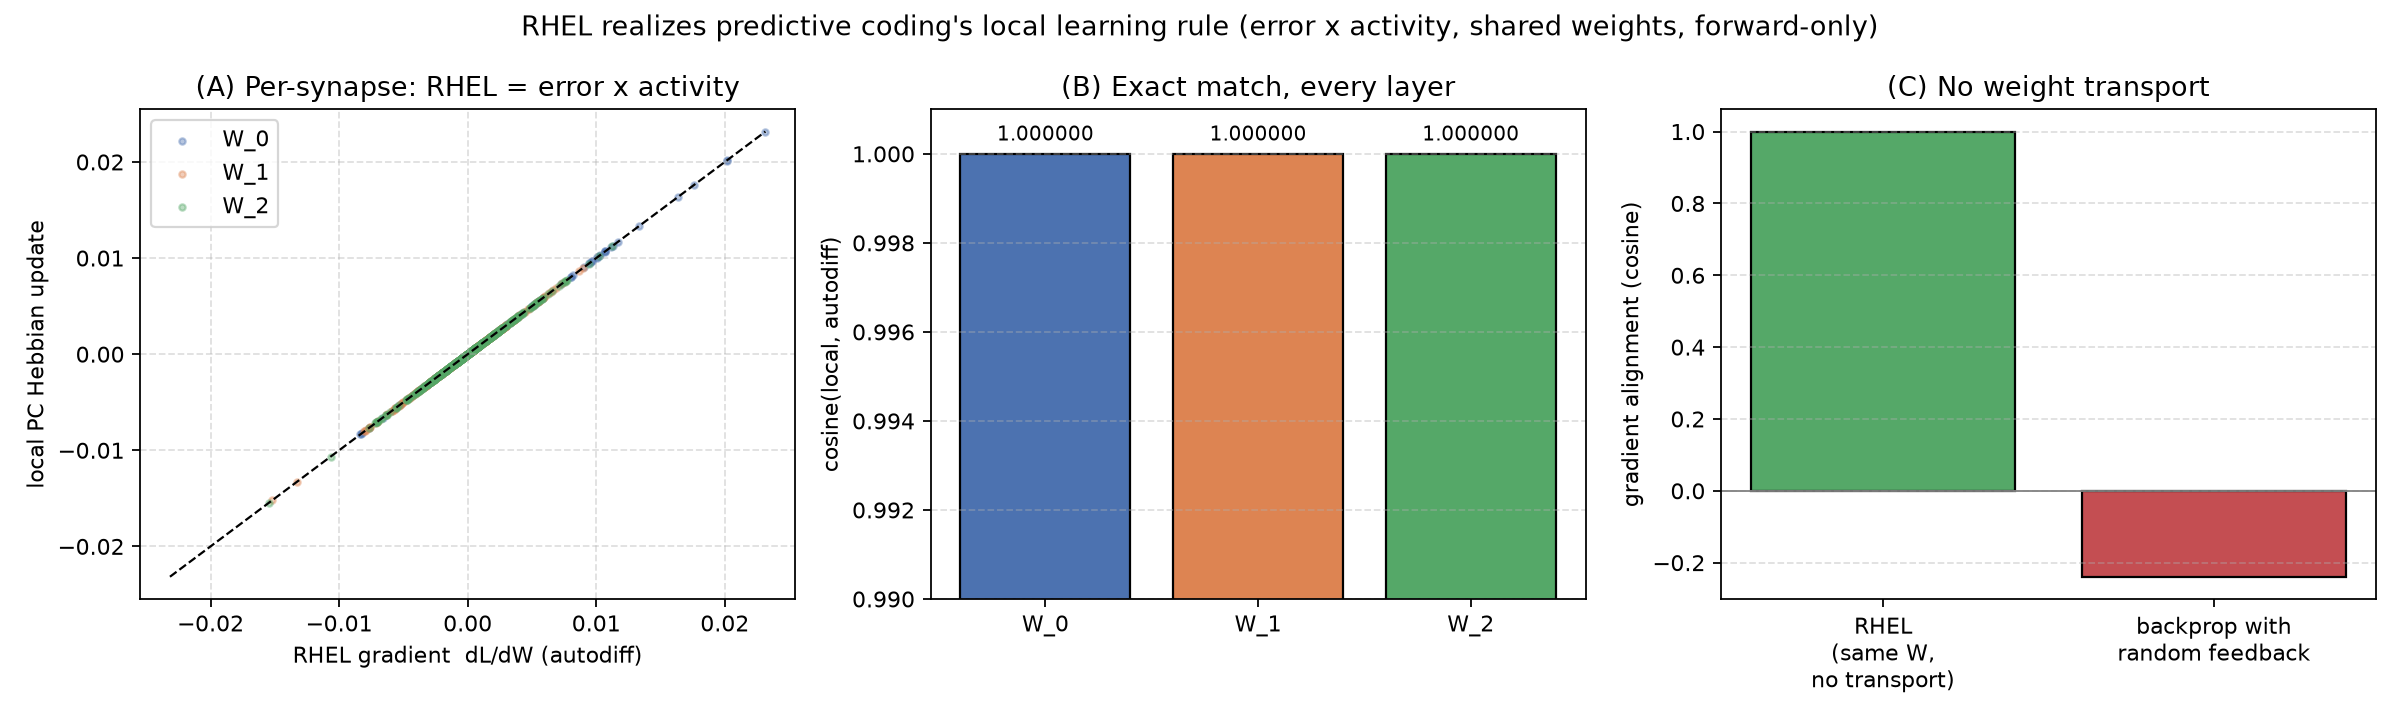
\includegraphics[width=\linewidth]{exp6_locality.png}
\caption{\textbf{RHEL realizes PC's local rule (benefit \#1).}
\emph{(A)} Per synapse, the hand-derived local error\,$\times$\,activity
update~\eqref{eq:hpc_update} lies on the $y\!=\!x$ line against the
autodiff RHEL gradient, every layer. \emph{(B)} Layer-wise cosine
similarity is $1.0$ (residual $\sim\!10^{-8}$). \emph{(C)} Backpropagation's
gradient \emph{depends} on transported weights: replacing the backward
weights with random ones (feedback-alignment control) misaligns it to cosine
$-0.24$, whereas RHEL reuses the forward weights and has nothing to
transport.}
\label{fig:locality}
\end{figure}

Proposition~\ref{prop:local} predicts that the RHEL update equals the local
PC rule at every synapse. Figure~\ref{fig:locality} confirms this: the
hand-written error\,$\times$\,activity contrast and the generic autodiff RHEL
gradient agree to cosine $1.0$ and maximum relative difference
$\sim\!10^{-8}$ across all layers (panels A--B). Panel~C quantifies the
significance of \emph{not} needing weight transport: standard backpropagation
through the inference dynamics uses the transposed weights in its backward
pass, and replacing them with fixed random matrices (the feedback-alignment
probe of \citealp{feedbackalignment}) misaligns the gradient to cosine
$-0.24$. RHEL's echo passes reuse the forward weights by construction, so
there is no separate backward weight to transport---HPC performs temporal
credit assignment with a fully local, weight-transport-free, forward-only
rule, and does so \emph{exactly} rather than approximately.

\subsection{Energy-based unsupervised learning}
\label{sec:unsup}

\begin{figure}[t]
\centering
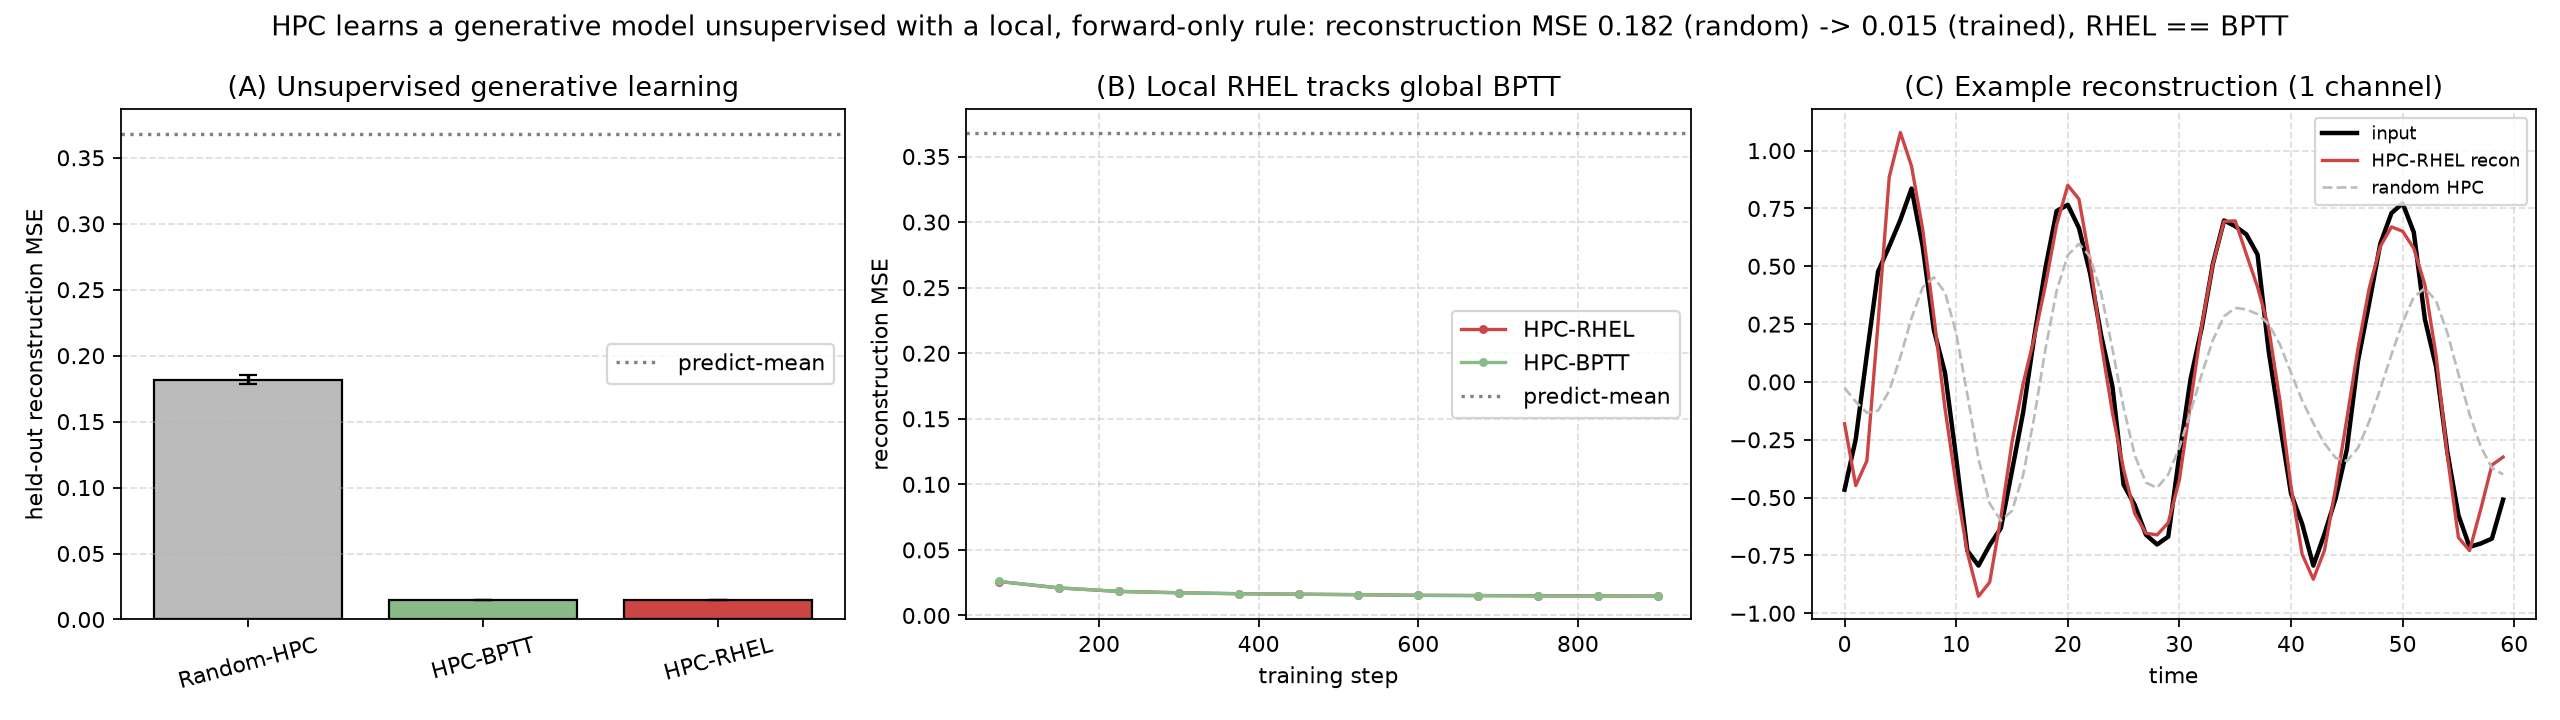
\includegraphics[width=\linewidth]{exp5_unsupervised.png}
\caption{\textbf{Unsupervised generative learning (benefit \#2).}
\emph{(A)} With no labels, HPC reduces held-out reconstruction error from
$0.182$ (random reservoir) to $0.015$, $25\times$ below predicting the mean.
\emph{(B)} The local RHEL rule and global BPTT produce identical
reconstruction-loss curves. \emph{(C)} A trained HPC reconstructs a held-out
waveform that the random reservoir cannot.}
\label{fig:unsup}
\end{figure}

Because PC is a generative model, HPC can learn without labels by minimizing
its free energy---the sensory prediction error---an objective a task-driven
sequence model does not possess. On a clean structured-waveform autoencoding
task (Fig.~\ref{fig:unsup}), unsupervised HPC reduces held-out reconstruction
mean-squared error from $0.182$ for a random Hamiltonian reservoir to $0.015$
after training ($12\times$ lower, $25\times$ below predicting the per-channel
mean), and a trained network reconstructs held-out waveforms that the random
reservoir cannot (panels A, C). Crucially, the \emph{local} RHEL rule and
\emph{global} BPTT yield reconstruction curves that coincide step for step
(panel B): locality costs nothing in optimization quality on the unsupervised
objective. We note two honest caveats in \S\ref{sec:limitations}: a weak leak
is required, and on this frequency-coded task a linear probe of the
representation saturates even for a random reservoir, so reconstruction---not
the probe---is the meaningful learning signal.

\subsection{The nudging knob: exact $\leftrightarrow$ robust}
\label{sec:knob}

\begin{figure}[t]
\centering
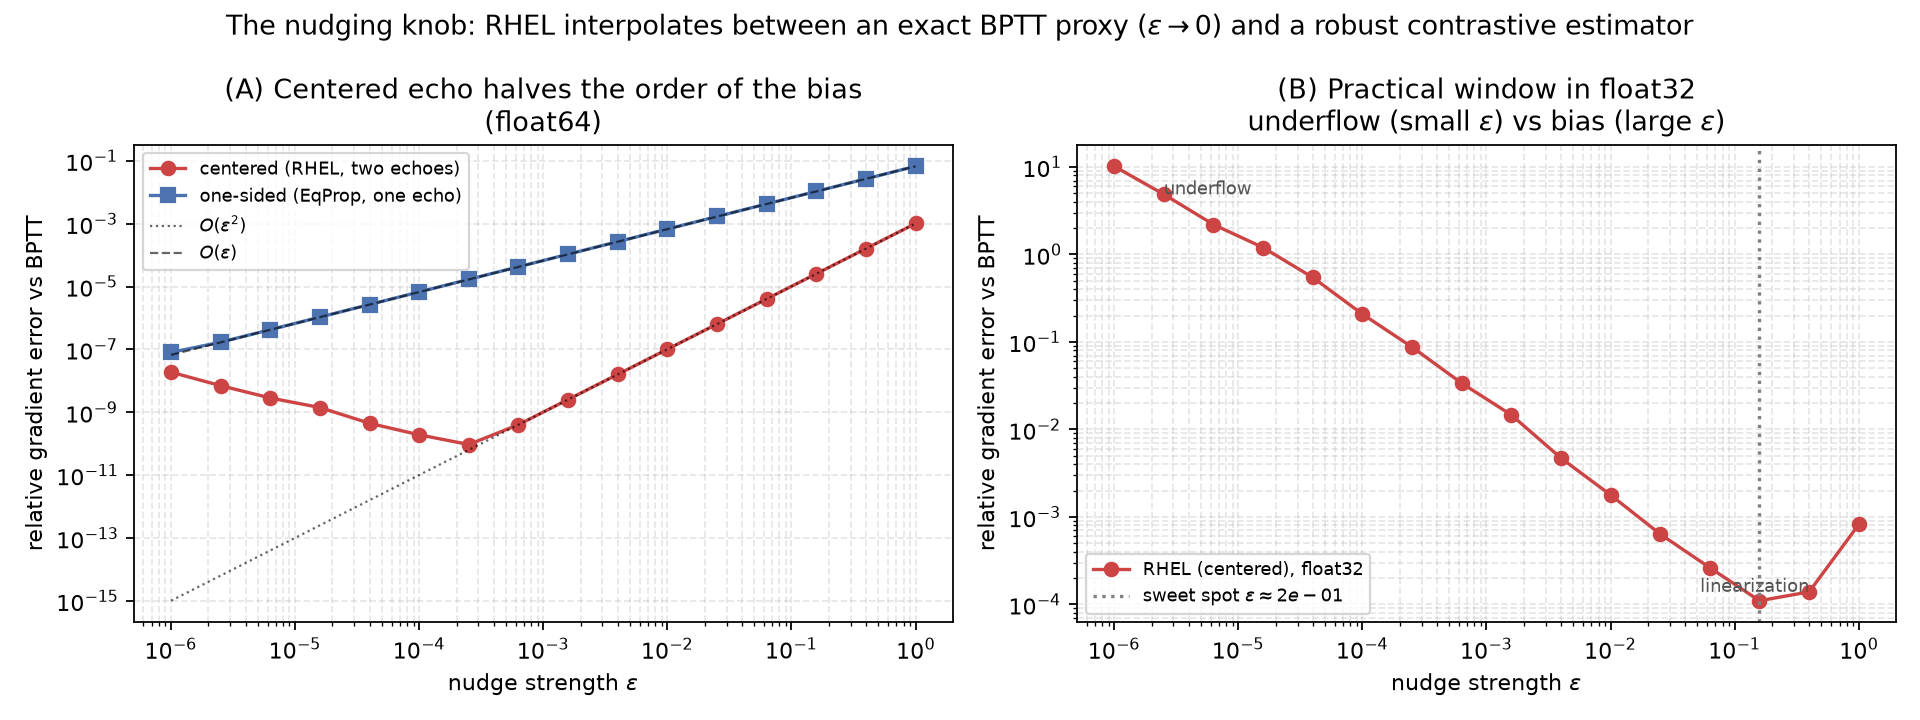
\includegraphics[width=\linewidth]{exp7_nudging_knob.png}
\caption{\textbf{The nudging knob.} \emph{(A, double precision)} RHEL's
centered two-echo estimator has $O(\eps^2)$ bias relative to BPTT; the
one-sided estimator (one echo, as in Equilibrium Propagation) has $O(\eps)$.
The symmetric echo buys one order of accuracy. \emph{(B, single precision)}
The $\eps\!\to\!0$ limit is unreachable (the perturbation underflows), so the
relative gradient error is U-shaped with a sweet spot near $\eps\!\approx\!0.1$,
the value used throughout.}
\label{fig:knob}
\end{figure}

RHEL's only approximation is the finite nudge $\eps$, making it a
one-parameter family between an exact BPTT proxy ($\eps\!\to\!0$) and a
biased but robust contrastive estimator---the regime it shares with
Equilibrium Propagation (EqProp; \citealp{eqprop}). Figure~\ref{fig:knob}A
shows that RHEL's \emph{centered} two-echo difference has $O(\eps^2)$ bias,
whereas a \emph{one-sided} nudge (the standard EqProp estimator: free state
plus one nudged state) has $O(\eps)$; flipping the momenta both ways buys an
extra order of accuracy. In single precision the small-$\eps$ limit is
unreachable because the $\eps$-perturbation underflows
(\citealp{rhel}, App.~A.5.4), producing a U-shaped error with a sweet spot
near $\eps\!\approx\!0.1$ (Fig.~\ref{fig:knob}B)---validating the nudging
strength used in all training runs.

\subsection{Does the finite-$\eps$ regime beat backpropagation? A negative result}
\label{sec:continual}

\begin{figure}[t]
\centering
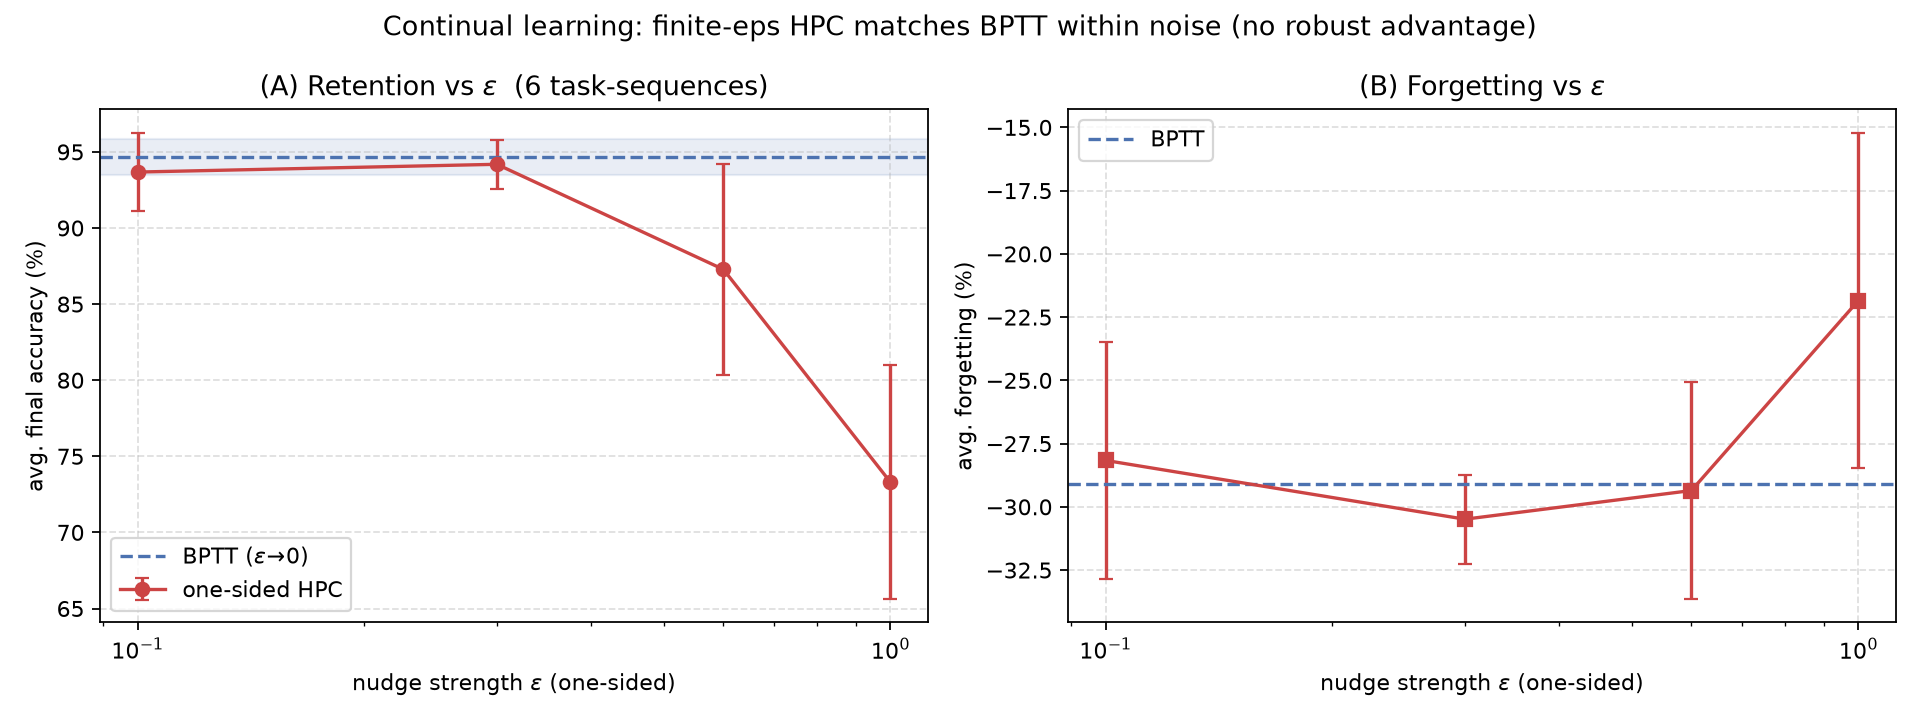
\includegraphics[width=\linewidth]{exp8_continual.png}
\caption{\textbf{No behavioral advantage over BPTT on continual learning.}
Domain-incremental sequence classification ($6$ tasks, shared model, $6$
task-sequences). \emph{(A)} Average final accuracy of one-sided HPC versus
nudge strength $\eps$; the $\eps\!\to\!0$ limit is BPTT (blue band: $\pm1$
s.d.). \emph{(B)} Forgetting. Small $\eps$ tracks BPTT within noise; large
$\eps$ degrades as the gradient bias dominates. The best non-zero $\eps$ wins
only $2/6$ task-sequences and loses on average.}
\label{fig:continual}
\end{figure}

A natural hypothesis is that the finite-$\eps$ regime---which updates weights
at \emph{target-nudged} activities, echoing predictive coding's ``prospective
configuration'' \citep{prospective}---should reduce catastrophic forgetting
relative to backpropagation. We test this directly with the one-sided
estimator, whose finite-$\eps$ bias is exactly such a prospective term, on a
domain-incremental continual-learning task (Fig.~\ref{fig:continual}), in a
fully matched comparison: same architecture, same data, only $\eps$ varies,
with $\eps\!\to\!0$ recovering BPTT. We find \emph{no robust advantage}.
Across six task-sequences, the best non-zero $\eps$ matches BPTT within seed
noise (and loses slightly on average), while large $\eps$ degrades retention
as the $O(\eps)$ gradient bias overwhelms any prospective effect. We report
this negative result deliberately: it confirms that HPC's value lies in
\emph{how} it assigns credit---locally, energy-based, forward-only, and
exactly equal to BPTT---not in superior task performance. It also localizes
where a genuine PC advantage must originate: in the \emph{equilibrium}
inference of dissipative PC, which conservative HPC forgoes for exactness.
Recovering that advantage without sacrificing locality---e.g.\ via controlled
dissipation---is the clearest direction this work opens (\S\ref{sec:limitations}).

\section{Related work}
\label{sec:related}
HPC sits at the intersection of three lines. \emph{Predictive coding}
\citep{raoballard,whittingtonbogacz,millidge_review} provides the local
error-driven objective; its relation to backpropagation is classically
asymptotic and inference-convergent, and recent work shows PC's
non-backprop inference can confer advantages such as ``prospective
configuration'' \citep{prospective}. \emph{Energy-based and equilibrium
learning}---Equilibrium Propagation \citep{eqprop,scellier_compare},
holomorphic EqProp \citep{holomorphic}, and self-learning Hamiltonian echo
backprop \citep{heb}---computes gradients through physical relaxation or
conservative dynamics; HPC inherits RHEL's extension of the latter to
sequences and losses defined over time, and instantiates it in the PC model
class where the learning rule becomes manifestly local. \emph{Hamiltonian and
state-space sequence models} \citep{linoss,unicornn,s4,mamba} supply the
recurrent backbone; we use a PC-structured Hamiltonian rather than a
task-tuned one. RHEL \citep{rhel} is our point of departure; we contribute the
PC instantiation, the locality/weight-transport analysis, the energy-based
unsupervised capability, and the centered-vs-one-sided bias result.

\section{Discussion and limitations}
\label{sec:limitations}
\textbf{Conservativity has a price.} Non-dissipative inference cannot forget:
energy injected by the input is never dissipated, so a strong leak collapses
the network to predicting the mean and a long noise-dominated history cannot
be selectively erased (consistent with the forgetting analysis of
\citealp{rhel}, App.~A.4.4). HPC therefore requires a weak leak and favors
tasks whose discriminative signal persists; controlled artificial dissipation
or inter-sequence resets are natural remedies and a clear direction for
future work. \textbf{Evaluation.} On our frequency-coded task a linear probe
saturates even for a random reservoir, so we report reconstruction quality,
not probe accuracy, as the unsupervised learning signal; harder
representation benchmarks are needed to separate learned from reservoir
features. \textbf{Scope.} Like RHEL, HPC is forward-only but not yet online
(inputs are replayed in reverse), still requires the explicit local gradient
$\grad_{\bW}F$ (benign for PC, but not fully ``black-box''), and matches
rather than beats BPTT on digital hardware; its promised advantage is for
analog physical substrates. We tested the most natural route to a behavioral
advantage---the prospective-configuration regime at finite $\eps$---and found
none (\S\ref{sec:continual}): HPC is engineered to be BPTT-exact, so the
accessible departures are either negligible or harmful. A genuine advantage
would have to come from \emph{equilibrium} (dissipative) inference, which
conservative HPC sacrifices for exactness; combining the two via controlled
dissipation, while preserving locality, is the central open problem.

\section{Conclusion}
\label{sec:conclusion}
Treating the predictive-coding free energy as the potential of a conservative
Hamiltonian turns the PC hierarchy into a single recurrent unit whose
inference is one symplectic forward pass and whose learning, via Recurrent
Hamiltonian Echo Learning, is exactly the local PC Hebbian rule computed
forward in time without weight transport. The same construction grants
energy-based unsupervised learning and a principled nudging knob bridging
exact backpropagation and Equilibrium Propagation. Hamiltonian predictive
coding is a step toward self-learning machines whose inference and plasticity
are one and the same physical process.

\small
\begin{thebibliography}{Whittington and Bogacz(2017)}
\bibitem[Pourcel and Ernoult(2025)]{rhel} G.~Pourcel and M.~Ernoult. Learning
long range dependencies through time reversal symmetry breaking.
\emph{NeurIPS}, 2025. arXiv:2506.05259.
\bibitem[Rao and Ballard(1999)]{raoballard} R.~P.~N. Rao and D.~H. Ballard.
Predictive coding in the visual cortex. \emph{Nature Neuroscience},
2(1):79--87, 1999.
\bibitem[Whittington and Bogacz(2017)]{whittingtonbogacz} J.~C.~R. Whittington
and R.~Bogacz. An approximation of the error backpropagation algorithm in a
predictive coding network. \emph{Neural Computation}, 29(5):1229--1262, 2017.
\bibitem[Millidge et al.(2022)]{millidge_review} B.~Millidge, A.~Tschantz, and
C.~L. Buckley. Predictive coding approximates backprop along arbitrary
computation graphs. \emph{Neural Computation}, 34(6):1329--1368, 2022.
\bibitem[Song et al.(2024)]{prospective} Y.~Song et al. Inferring neural
activity before plasticity as a foundation for learning beyond
backpropagation. \emph{Nature Neuroscience}, 27:348--358, 2024.
\bibitem[Scellier and Bengio(2017)]{eqprop} B.~Scellier and Y.~Bengio.
Equilibrium propagation: bridging the gap between energy-based models and
backpropagation. \emph{Frontiers in Computational Neuroscience}, 11:24, 2017.
\bibitem[Scellier et al.(2023)]{scellier_compare} B.~Scellier, M.~Ernoult,
J.~Kendall, and S.~Kumar. Energy-based learning algorithms for analog
computing: a comparative study. \emph{NeurIPS}, 2023.
\bibitem[Laborieux and Zenke(2022)]{holomorphic} A.~Laborieux and F.~Zenke.
Holomorphic equilibrium propagation computes exact gradients through finite
size oscillations. \emph{NeurIPS}, 2022.
\bibitem[Lopez-Pastor and Marquardt(2023)]{heb} V.~Lopez-Pastor and
F.~Marquardt. Self-learning machines based on Hamiltonian echo
backpropagation. \emph{Physical Review X}, 13(3):031020, 2023.
\bibitem[Lillicrap et al.(2016)]{feedbackalignment} T.~P. Lillicrap,
D.~Cownden, D.~B. Tweed, and C.~J. Akerman. Random synaptic feedback weights
support error backpropagation for deep learning. \emph{Nature
Communications}, 7:13276, 2016.
\bibitem[Rusch and Rus(2024)]{linoss} T.~K. Rusch and D.~Rus. Oscillatory
state-space models. arXiv:2410.03943, 2024.
\bibitem[Rusch and Mishra(2021)]{unicornn} T.~K. Rusch and S.~Mishra.
UnICORNN: a recurrent model for learning very long time dependencies.
\emph{ICML}, 2021.
\bibitem[Gu et al.(2022)]{s4} A.~Gu, K.~Goel, and C.~R\'e. Efficiently
modeling long sequences with structured state spaces. \emph{ICLR}, 2022.
\bibitem[Gu and Dao(2023)]{mamba} A.~Gu and T.~Dao. Mamba: linear-time
sequence modeling with selective state spaces. arXiv:2312.00752, 2023.
\bibitem[Momeni et al.(2024)]{physnn} A.~Momeni et al. Training of physical
neural networks. arXiv:2406.03372, 2024.
\bibitem[Hooker(2021)]{hardwarelottery} S.~Hooker. The hardware lottery.
\emph{Communications of the ACM}, 64(12):58--65, 2021.
\end{thebibliography}

\appendix
\section{Model and experimental details}
\label{app:details}
\paragraph{Hamiltonian and integrator.} With the time step $\delta$ folded
into $H$ (so the leapfrog runs at unit step), the HPC potential is
$V[\bz]=\delta\big(\sum_\ell\half\|\mathbf{e}_\ell\|^2+\tfrac{\alpha}{2}\|\bz\|^2\big)$
with errors~\eqref{eq:errors}, and $T[\bpi]=\delta\,\half\|\bpi\|^2$. The
leapfrog map updates position by a half step, momentum by a full step using
$-\grad_{\bz}V$, then position by a half step; the RHEL gradient is read at
the intermediate half-step positions.

\paragraph{Networks and training.} Unless noted, $L=3$ levels and width $16$--$32$.
The unsupervised experiments use $\delta=0.5,\ \alpha=0.05$ (a weak leak so
latents track the input); the supervised and locality experiments use
$\delta\in[0.1,0.2],\ \alpha\in[0.1,0.3]$. Optimization is Adam; RHEL uses
$\eps=0.1$ with the loss rescaling $\gamma$ of \citet{rhel} (we find
$\gamma\approx10^2$ optimal for HPC, versus $10^4$ for the larger
state-space models, because the PC loss magnitudes differ---one must regrid
$\gamma$ per model). The readout head (per-step linear map, $\tanh$, temporal
mean-pool, linear decoder) is differentiated by autodiff and chained with
RHEL at the HRU boundary. A dissipative-PC baseline relaxes the same free
energy for $40$ steps and applies~\eqref{eq:pc_hebb} at the relaxed state.

\paragraph{Reproducibility.} All experiments and figures are produced by the
scripts \texttt{exp4\_hpc\_prototype.py} (exactness, supervised),
\texttt{exp6\_locality.py} (Fig.~\ref{fig:locality}),
\texttt{exp5\_unsupervised.py} (Fig.~\ref{fig:unsup}), and
\texttt{exp7\_nudging\_knob.py} (Fig.~\ref{fig:knob}); the underlying RHEL
machinery (leapfrog HRU and custom-VJP echo backward pass) and the
Hamiltonian PC model are in the accompanying code.

\end{document}
